\documentclass[12pt, a4paper]{article}
\usepackage[margin = 1in, top=1.3in]{geometry}
\usepackage[english]{babel}
\usepackage[utf8]{inputenc}
\usepackage{fancyhdr}
\usepackage[fleqn]{amsmath}
\usepackage{mathtools}
\usepackage{tabto}
\usepackage{bm}
\usepackage{graphicx}
\graphicspath{{./images/}}
\usepackage[font=small,labelfont=bf]{caption}
 
\pagestyle{fancy}
\fancyhf{}
\rhead{\small{Shaan Ul Haque(180070053)\\ Samarth Singh (180050090) \\ Niraj Mahajan (180050069)}}
\lhead{CS-663 Assignment-2 : Question 3}
\rfoot{Page 3.\thepage}
 
\begin{document}
\vspace*{-22pt}
\section*{Question 3}
\subsection*{3.1 Isotropic Gaussian Mask}
We used a gaussian mask of $\sigma$ = 1.5 to make the patches isotropic.
\renewcommand{\thefigure}{3.1}
\begin{figure}[h]
    \centering
    \vspace*{-15pt}
    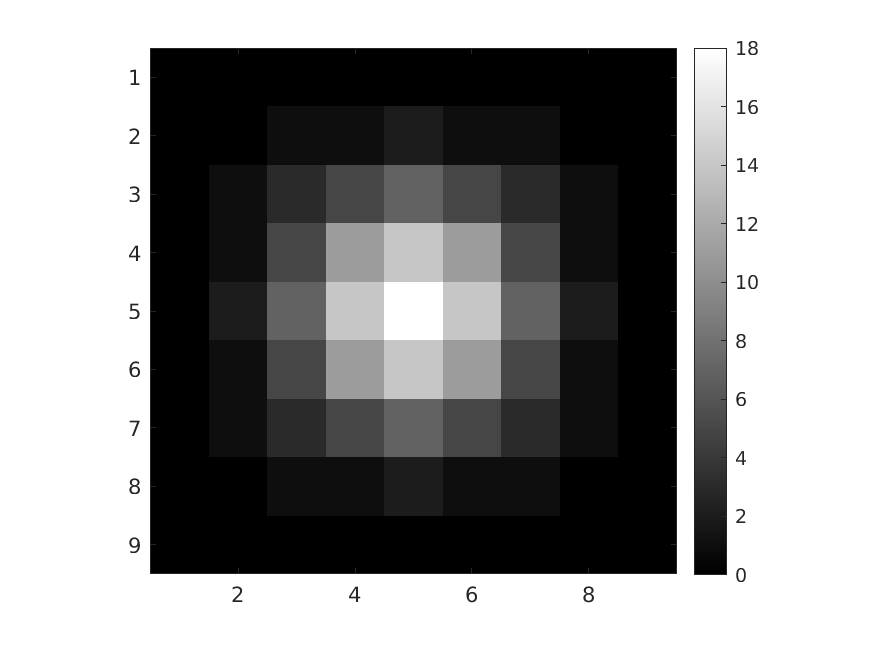
\includegraphics[width=0.5\textwidth]{isotropic_filter.png}
    \vspace*{-15pt}
    \caption{Gaussian Mask}
    \label{fig:2.6}
\end{figure}

\subsection*{3.2 Patch Based Filtering on barbara.png}
\noindent The optimal filtering for barbara.png was attained at $\sigma_{barbara} = 0.8424$. \\
The RMSD values are:
\begin{itemize}
	\item RMSD$_{\sigma}\;\;\;$  = 2.614193
	\item RMSD$_{0.9\sigma}$ = 2.669242
	\item RMSD$_{1.1\sigma}$ = 2.636064
\end{itemize}
\begin{figure}[h]
    \centering
    \renewcommand{\thefigure}{3.2(a)}
    \begin{minipage}[c][1\width]{0.3\textwidth}
    	\hspace*{-1in}
    	\includegraphics[width=1.5\textwidth]{barbara_original.png}
    	\caption{Original}
	    \label{fig:3.2(a)}
    \end{minipage}
    \renewcommand{\thefigure}{3.2(b)}
    \begin{minipage}[c][1\width]{0.3\textwidth}
    	\hspace*{-0.5in}
    	\includegraphics[width=1.5\textwidth]{barbara_corrupted.png}
    	\caption{Corrupted}
	    \label{fig:3.2(b)}
    \end{minipage}
    \renewcommand{\thefigure}{3.2(c)}
    \begin{minipage}[c][1\width]{0.3\textwidth}
    	\includegraphics[width=1.5\textwidth]{barbara_filtered.png}
    	\caption{Filtered}
	    \label{fig:3.2(c)}
    \end{minipage}
\end{figure}
\newpage
\subsection*{3.3 Patch Based Filtering on grass.png}
\noindent The optimal filtering for barbara.png was attained at $\sigma_{grass} = 1.81$. \\
The RMSD values are:
\begin{itemize}
	\item RMSD$_{\sigma}\;\;\;$  = 7.265757
	\item RMSD$_{0.9\sigma}$ = 7.303963
	\item RMSD$_{1.1\sigma}$ = 7.520618
\end{itemize}
\begin{figure}[h]
    \centering
    \renewcommand{\thefigure}{3.3(a)}
    \begin{minipage}[c][1\width]{0.3\textwidth}
    	\hspace*{-1in}
    	\includegraphics[width=1.5\textwidth]{grass_original.png}
    	\caption{Original}
	    \label{fig:3.3(a)}
    \end{minipage}
    \renewcommand{\thefigure}{3.3(b)}
    \begin{minipage}[c][1\width]{0.3\textwidth}
    	\hspace*{-0.5in}
    	\includegraphics[width=1.5\textwidth]{grass_corrupted.png}
    	\caption{Corrupted}
	    \label{fig:3.3(b)}
    \end{minipage}
    \renewcommand{\thefigure}{3.3(c)}
    \begin{minipage}[c][1\width]{0.3\textwidth}
    	\includegraphics[width=1.5\textwidth]{grass_filtered.png}
    	\caption{Filtered}
	    \label{fig:3.3(c)}
    \end{minipage}
\end{figure}

\subsection*{3.4 Patch Based Filtering on beehive.png}
\noindent The optimal filtering for barbara.png was attained at $\sigma_{beehive} = 2.1$. \\
The RMSD values are:
\begin{itemize}
	\item RMSD$_{\sigma}\;\;\;$  = 7.432849
	\item RMSD$_{0.9\sigma}$ = 7.578823
	\item RMSD$_{1.1\sigma}$ = 7.559053
\end{itemize}
\begin{figure}[h]
    \centering
    \renewcommand{\thefigure}{3.4(a)}
    \begin{minipage}[c][1\width]{0.3\textwidth}
    	\hspace*{-1in}
    	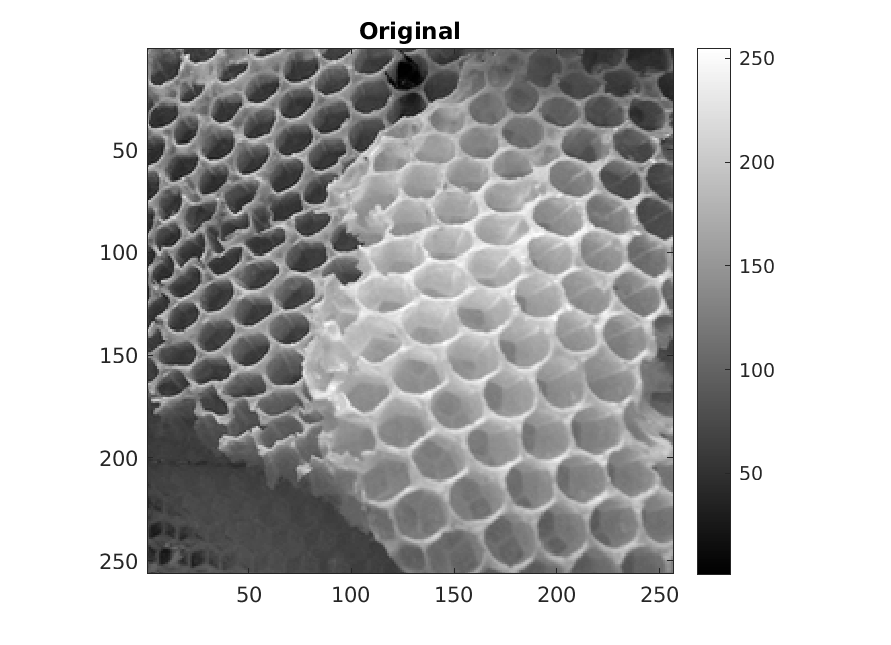
\includegraphics[width=1.5\textwidth]{Honeycomb_original.png}
    	\caption{Original}
	    \label{fig:3.4(a)}
    \end{minipage}
    \renewcommand{\thefigure}{3.4(b)}
    \begin{minipage}[c][1\width]{0.3\textwidth}
    	\hspace*{-0.5in}
    	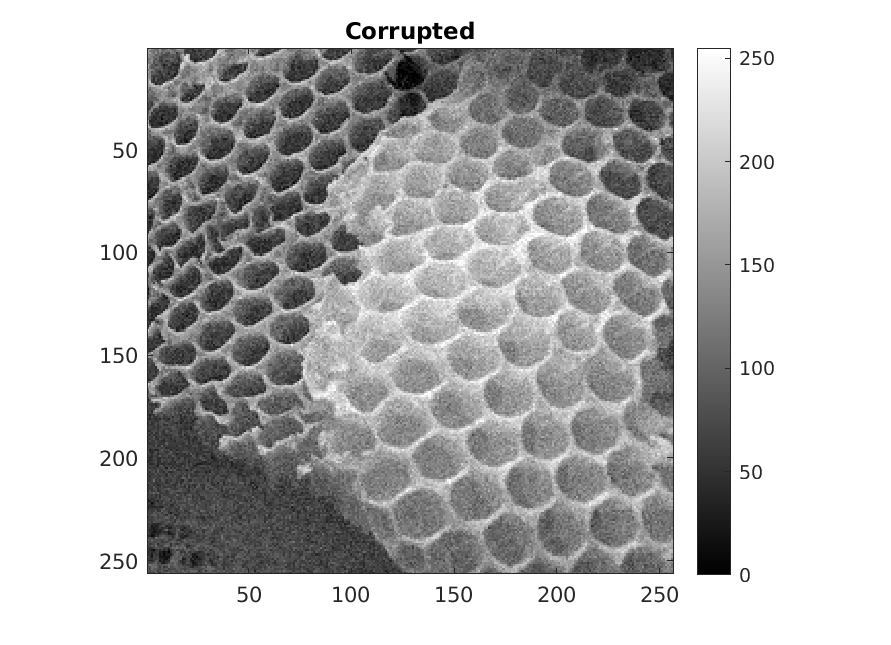
\includegraphics[width=1.5\textwidth]{Honeycomb_corrupted.png}
    	\caption{Corrupted}
	    \label{fig:3.4(b)}
    \end{minipage}
    \renewcommand{\thefigure}{3.4(c)}
    \begin{minipage}[c][1\width]{0.3\textwidth}
    	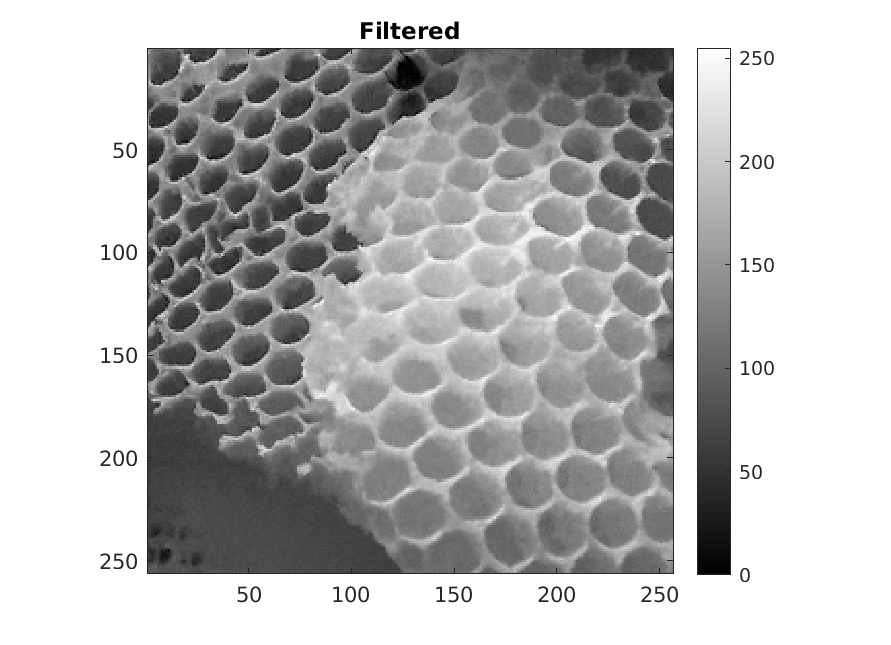
\includegraphics[width=1.5\textwidth]{Honeycomb_filtered.png}
    	\caption{Filtered}
	    \label{fig:3.4(c)}
    \end{minipage}
\end{figure}

\end{document}